

\documentclass[fleqn, 12pt]{article}
\usepackage[T1]{fontenc}
\usepackage{tocloft}
\usepackage[margin=1.1in]{geometry} 
\usepackage{amsmath,amsthm,amssymb,amsfonts, fancyhdr, color, comment, graphicx, environ}
\usepackage{xcolor}
\usepackage{mdframed}
\usepackage{graphicx}
\usepackage{caption}
\usepackage{subcaption}
\usepackage[shortlabels]{enumitem}
\usepackage{indentfirst}
\usepackage{hyperref}
\usepackage[serbian]{babel}
\renewcommand{\footrulewidth}{1 pt}
\usepackage{cite}
\bibliographystyle{plain}
\usepackage{float}

\hypersetup{
    colorlinks=true,
    linkcolor=blue,
    filecolor=magenta,      
    urlcolor=blue,
}


\pagestyle{fancy}



\newenvironment{problem}[2][Problem]
    { \begin{mdframed}[backgroundcolor=gray!20] \textbf{#1 #2} \\}
    {  \end{mdframed}}


\newenvironment{solution}{\textbf{Solution}}


\lhead{Aleksa Jovanović}
\rhead{Računarstvo i društvo} 
\chead{\textbf{}}
\lfoot{Prof. Sana Stojanović Đurđević}
\rfoot{Matematički fakultet, Beograd}

\renewcommand{\contentsname}{Sadržaj}
\begin{document}
\title{\Large Kurs: Računarstvo i društvo  \\[0.5cm]
        \bf\Large Bezbednost naših lozinki}
\author{\large Autor: Aleksa Jovanović\\ \ \\}
\date{\large Datum: \today}

\makeatletter
    \begin{titlepage}
        \begin{center}
	    {\ \\ \ \\}
        \vbox{}\vspace{5cm}
            {\@title }\\[3cm] 
            {\@author}
            {\large Predmetni profesor: \bf Prof. Sana Stojanović Đurđević\\  \ \\}
            {\@date\\}

        \end{center}
    \end{titlepage}
\makeatother

\setcounter{tocdepth}{2}
\tableofcontents

\newpage

\section{Uvod}
\indent Korišćenje šifara u današnjem digitalnom svetu je (trenutno) nezaobilazna realnost i prva linija odbrane od neželjenog pristupa našim profilima, podacima, finansijama i komunikacijama. Sigurnost celokupnog sistema je jaka samo koliko i najslabija karika, koja je pretežno korisnik. Loše prakse pri kreiranju i čuvanju lozinki, i korišćenju interneta olakšavaju zlonamernim akterima pristup privatnim podacima. Ovaj rad će se stoga glavno fokusirati na uvid u potencijalnu štetu koja može biti naneta, prvenstveno na individualnom nivou, kao i na predloge korekcija loših praksa. 

Sekcija 2 je fokusirana na posledice slabih lozinki i potencijalnih postupaka napadača nakon što dobiju pristup nalogu. Metodi razotkrivanja šifara, loše korisničke prakse i mere prevencija su predstavljeni u sekcijama 3 i 4. Dodatni metodi zaštite naloga, njihove prednosti i mane su razrađeni u sekciji 5. 

\section{Uticaj na druge sfere života}

\subsection{Privatnost na internetu}
\indent Pristup nalozima omogućava zlonamernim akterima da nanesu društvenu štetu žrtvi. Neki od mogućih načina su postavljanje neprimernog sadržaja, obmanljivo slanje privatnih poruka, čitanje i dokumentovanje privatnih poruka.

\subsection{Spam}
\indent Kompromitovani nalozi su mnogo efikasniji u širenju spam poruka. Sama dinamika širenja tih spam poruka je drugačija od dinamike širenja ``tradicionalnih'' spam poruka. Ovo je posledica toga što primalac te poruke ima iluziju da je poruka poslata od osobe od poverenja, što povećava šansu da i oni sami dalje prošire taj spam. Potpuna automatizacija pomenutog procesa omogućava veoma agresivnu propagaciju. \cite{spam}
Ovaj tip spama često širi i maliciozne linkove koji kompromituju naloge, što ih uvodi u svoju ``mrežu botova''.

\subsection{Žene kao mete sajber napada}
\indent Žene su češće mete nefinansijski motivisanih sajber napada poput desimenacije osvetničke pornografije, sajber uhođenja i krađe identiteta. Pored toga, procentualno više žena (u poređenju sa muškarcima) se oseća manje sigurno (35\% i 27\%, respektivno) i manje privatno (53\% i 47\%, respektivno). \cite{zene} \cite{zene2}


\newpage
\section{Česti napadi i greške korisnika}

\subsection{Napad grubom silom}
\indent Jedan od najosnovnijih napada koji se oslanja na naivno nagađanje šifara kombinovanjem datih karaktera. Glavni adut je jednostavnost implementacije. Ako je dužina šifre nepoznata, započinje se minimalnom dužinom šifre koja se inkrementira nakon iscrpljenja svih kombinacija za tu dužinu, ako nije došlo do pogotka.\cite{napadi}

\subsection{Napad rečnikom}
\indent Kolekcija reči se koristi za genersianje potencijalnih šifara. Rečnici mogu da budu opšte namene (npr. najčešće reči, imena i prezimena nekog jezika) ili specijalizovani (dodate su prethodno razotkrivene šifre iz skupa šifara koji je napadnut). U rečnike su često dodate sve kombinacije slova, brojeva i specijalnih karaktera do neke predodređene dužine. \cite{napadi}

\subsection{Ponovno korišćenje šifara}
\indent Česta (loša) praksa je ponovno korišćenje šifara zarad lakšeg pamćenja. Otkrivanje šifre jednog naloga je dovoljno za otkrivanje šifara svih ostalih naloga. Slično tome, male varijacije šifre za različite naloge se smatraju nesigurnim.

\subsection{Ostale loše prakse}
\indent Neredovno ažuriranje lozinki i njihovo nesigurno čuvanje su takođe faktori koji utiču na sveukupnu sigurnost lozinki. Nesigurno čuvanje podrazumeva njihovo zapisivanje na lako dostupinim papirima ili u neenkriptovane fajlove. Neuažuriranje šifara čini naloge podložne napadima koji koriste prethodna curenja podataka. 

Načini čuvanja šifara ne variraju značajno među demografijama, što nagoveštava  da nivo tehnološkog obrazovanja nije značajan indikator o korišćenju sigurnijih metoda. \cite{pew1}  
\begin{figure}[H]
    \centering
    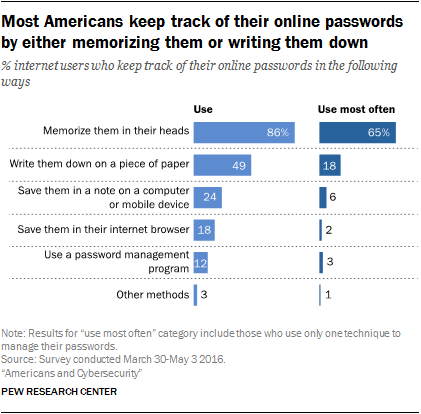
\includegraphics[width=0.5\linewidth]{pew.png}
    \caption{Načini pamćenja šifara građana SAD-a.\cite{pew1}}
    \label{fig:enter-label}
\end{figure}

\section{Mere prevencije}
\subsection{Jačina lozinki}
\indent Smanjivanje uspešnosti napada grubom silom se dostiže korišćenjem većeg skupa karaktera i dužih reči. Primera radi, postoji 4096000000 mogućih šifara od 6 karaktera i skupom karaktera koji čine mala slova azbuke i cifre od 0 do 9. Korišćenjem extended ASCII karaktera i šifru dužine 15, dobijamo 1.329228e+36 mogućih šifara. 

Osiguravanje od napada rečnikom se može izvesti na dva načina:
\begin{itemize}
    \item Izbegavanje korišćenja reči u lozinci. Lozinka bi sadržala veliki broj nasumično generisanih karaktera.
    \item Veliki broj reči koji formira ``frazu lozinke''.
\end{itemize}

\subsection{Alati}
\indent Da bi se pojednostavio proces generisanja jakih nasumičnih lozinki i njihovo sigurno skladištenje, koriste se menadžeri lozinki (eng. \emph{password manager}) poput KeePassXC i Buttercup. 

KeePassXC je alat otvorenog koda za enkriptovanje skladištenje i upravljanje korisničkim imenima, šiframa, linkovima i prioleženim fajlovima. Ne postoji ugrađena mogućnost sinhronizacije baze između većeg broja uređaja, ali je korisnicima dozvoljeno i učinjeno jednostavnim da sami urade rešenje po želji. \cite{keepassxc}

U odnosu na KeePassXC, Buttercup ima moderniji interfejs i ugrađenu podršku za sinhronizaciju baze. \cite{buttercup}


\begin{figure}[h]
    \centering
    \begin{subfigure}[b]{0.45\linewidth}
        \centering
        
\includegraphics[width=\linewidth]{keepassXC_logo.png}
        \caption{KeePassXC logo}
        \label{fig:image1}
    \end{subfigure}
    \hfill
    \begin{subfigure}[b]{0.45\linewidth}
        \centering
        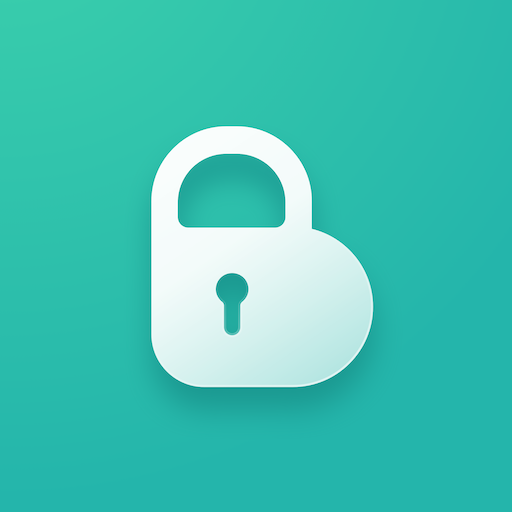
\includegraphics[width=\linewidth]{buttercup_logo.png}
        \caption{Buttercup logo}
        \label{fig:image2}
    \end{subfigure}
    \caption{}
    \label{fig:side_by_side}
\end{figure}

\newpage
\section{Alternative i dodatna zaštita}
\indent Korišćenje samo šifre često nije dovoljno, te se koriste dotatne mere: 2FA, Yubikey, sigurnosna pitanja, biometrijska autentikacija. Kombinacija ovih mera čini kompromitovanje naloga značajno težim, ali takođe stvara dodatno trenje između korisnika i pristupa njihovom nalogu. Ovo trenje, kao i trenje koje nastaje pri korišćenju menadžera lozinki, je razlog za česte loše prakse kod velikog broja korisnika. Trenutni cilj eksperata sajber sigurnosti nije samo edukacija što šire publike, nego i konstrukcija sigurnih sistema sa minimalnim trenjem. 

\subsection{Jednokratne lozinke}
Jedan od najčešćih oblika MFA je OTP (jednokratne lozinke, eng. \emph{one time passwords}). Korisnici mogu da pristupe jednokratnim lozinkama korišćenjem aplikacija (poput 2FAS ili Aegis Authenticator) ili da im budu dostavljene SMS porukama. Lozinke su generisanje korišćenjem konstantog seed-a i pomerajućeg faktora.\cite{OTP} Varijante OTP-a se dele po načinu generisanja pomerajućeg faktora:
\begin{itemize}
    \item HOTP (eng. \emph{Hash-based Message Authentication Code One Time Password})
    \item TOTP (eng. \emph{Time-based One-time Password})
\end{itemize}

Osnovna ideja iza HOTP je baziranje pomerajućeg faktora na brojaču koji prati broj zahtevanih lozinki. 

\begin{figure}[H]
    \centering
    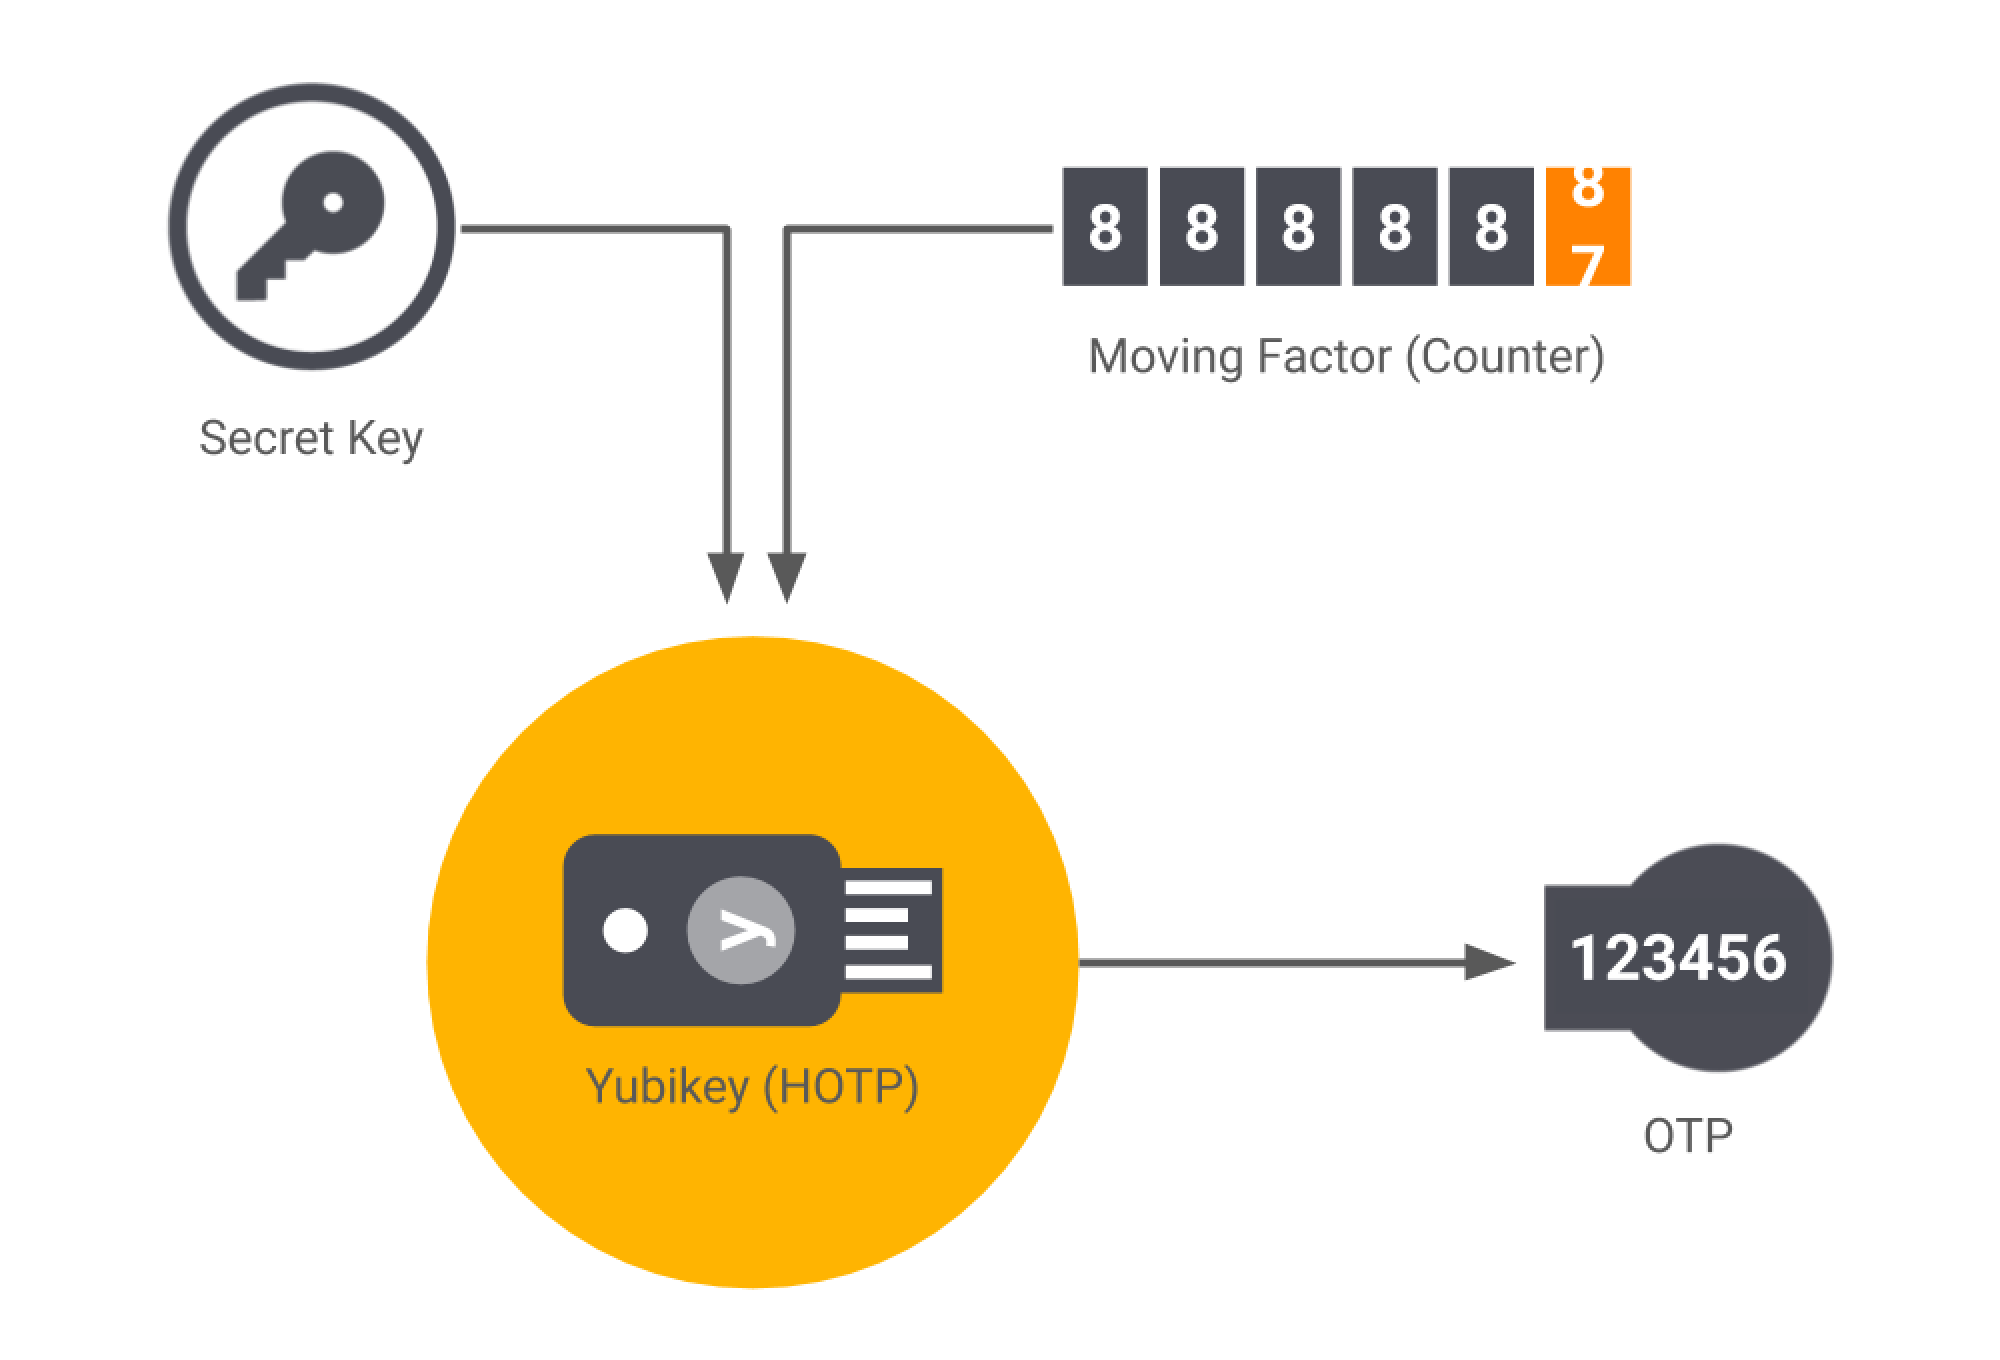
\includegraphics[width=0.5\linewidth]{HOTP.png}
    \caption{Shema rada HOTP sistema.\cite{OTP}}
    \label{fig:enter-label}
\end{figure}

Za razliku od ovog pristupa, TOTP koristi vreme zahteva kao pomerajući faktor. Vremenski korak uglavnom iznosi između 30 i 60 sekundi i ako lozinka nije iskorišćena tokom tog vremena ona prestaje da bude validna. U tom slučaju, potrebno je zahtevati novu lozinku. 

\begin{figure}[H]
    \centering
    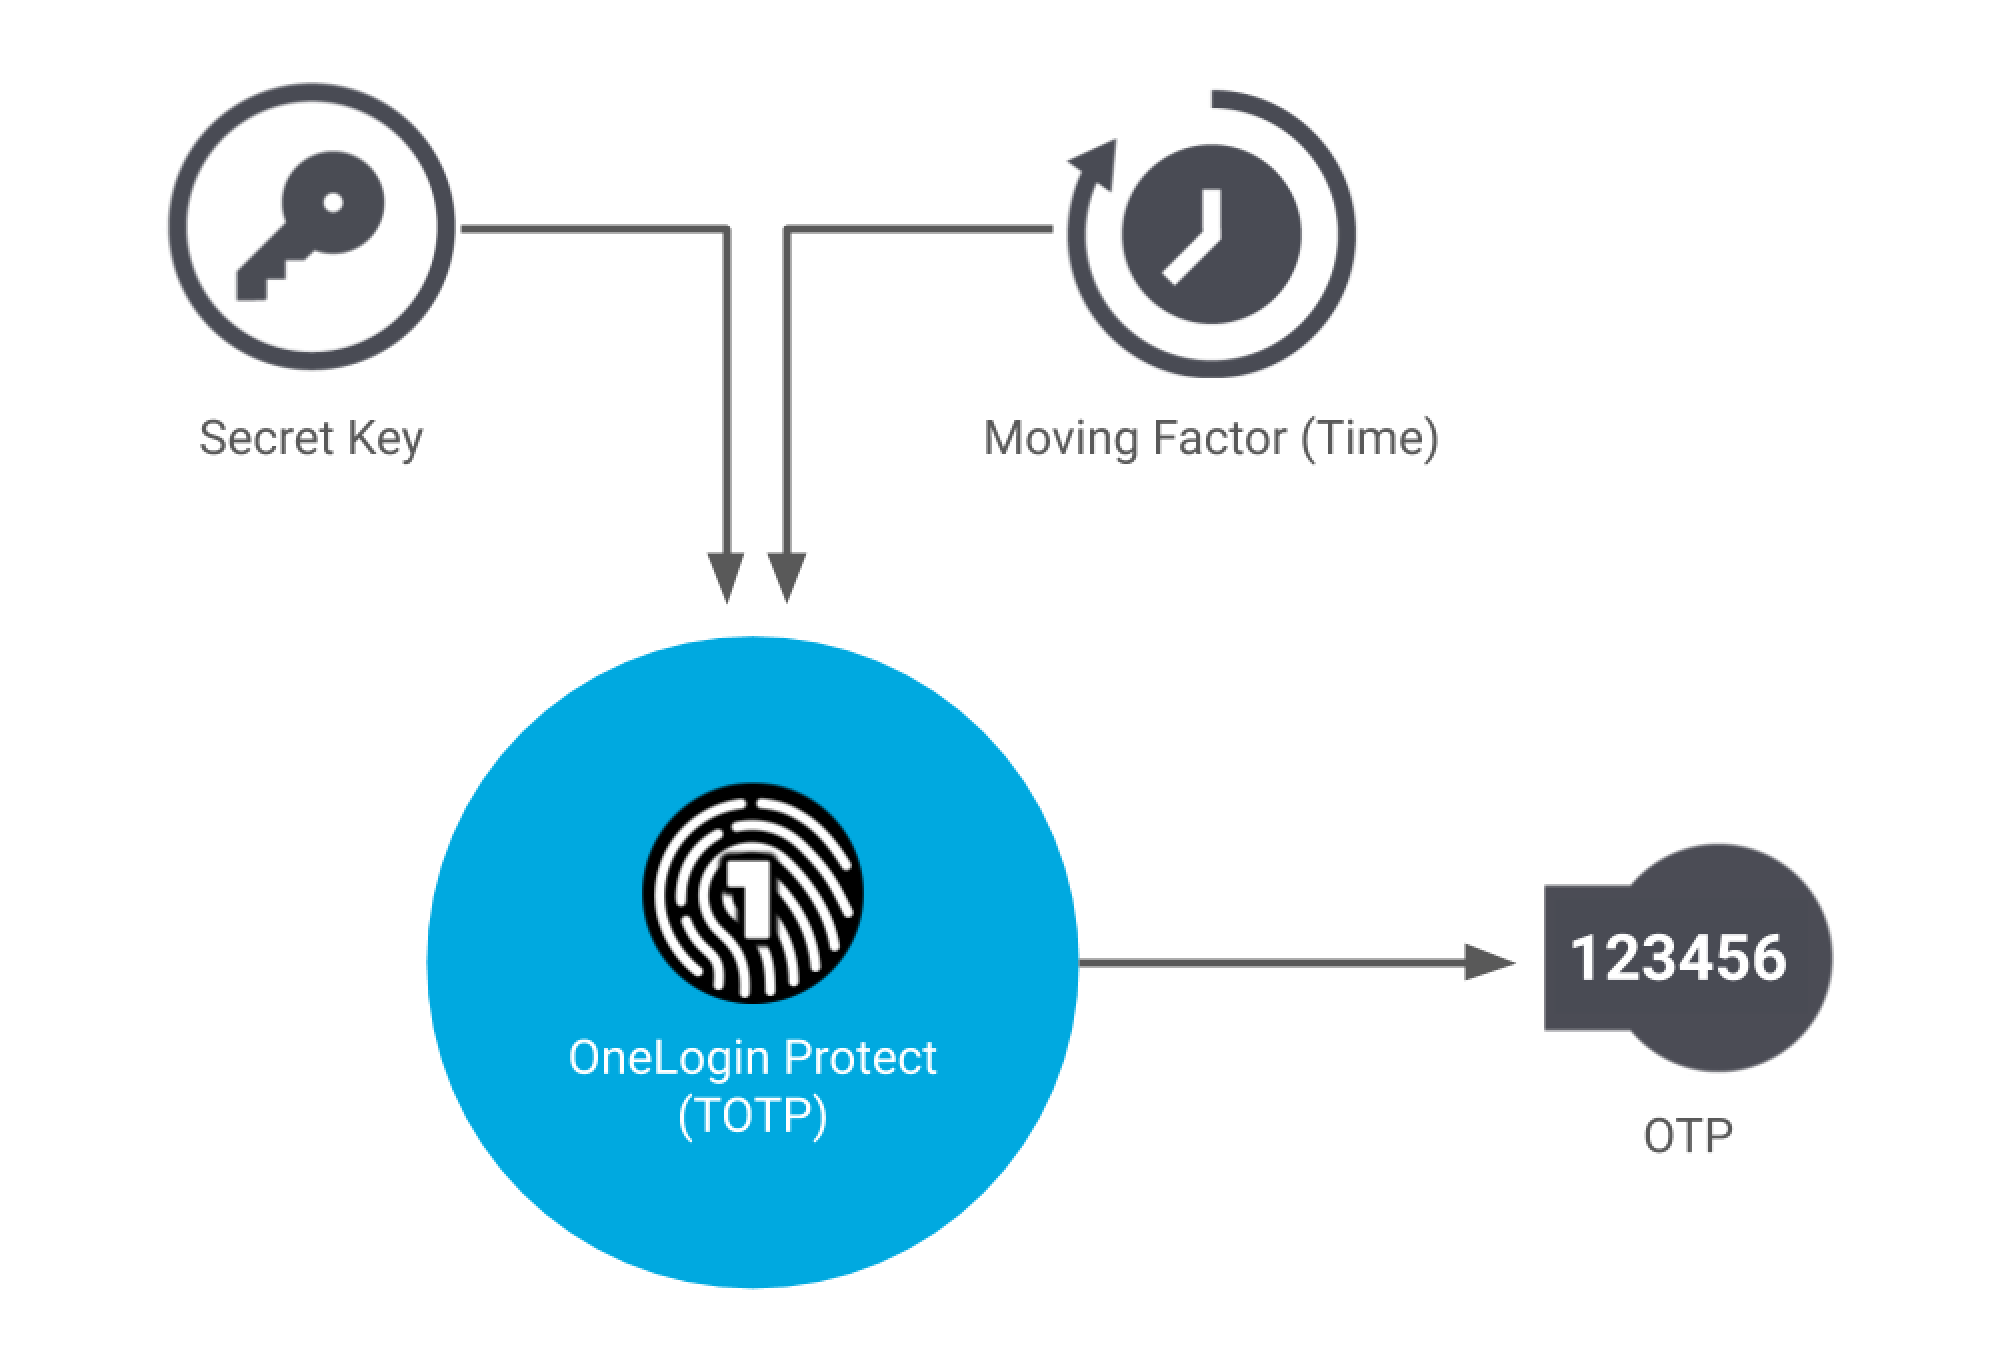
\includegraphics[width=0.5\linewidth]{TOTP.png}
    \caption{Shema rada TOTP sistema.\cite{OTP}}
    \label{fig:enter-label}
\end{figure}

Koriščenje aplikacija od poverenja za pristup jednokratnim lozinkama je sigurnije od korišćenje SMS poruka, zbog podložnosti SMS poruka napadima poput man-in-the-middle napadu.

\newpage
\subsection{Biometrijska autentikacija}
\indent Način verifikacije identiteta korišćenjem bioloških karakteristika ili ponašanja korisnika. Biološke karakteristike korišćene za verifikaciju su:
\begin{itemize}
    \item Sken mrežnjače
    \item Sken otiska prsta
    \item Sken lica
    \item Poklapanje DNK 
\end{itemize}

Ponašanje korisnika uključuje navike korišćenja miša, tastature ili tač-skrina, koje su analizirane i poređene sa standardnim navikama. 

Korišćenje biometrijskih metoda autentikacije se ne sme smatrati stopostotno sigurnim, nego samo još jednim delom MFA lanca. Moguće je rekreirati neke od bioloških karakteristika, što potpuno negira prednosti koje ovaj vid zaštite donosi. \cite{bio}

\begin{figure}[H]
    \centering
    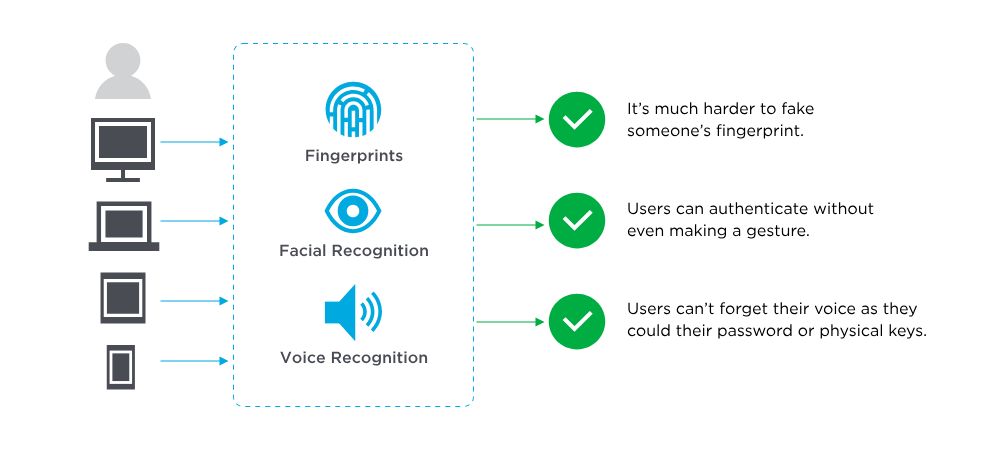
\includegraphics[width=1\linewidth]{bio.png}
    \caption{Pozitivne strane biometrijske autentikacije.\cite{bio}}
    \label{fig:enter-label}
\end{figure}

\begin{figure}[H]
    \centering
    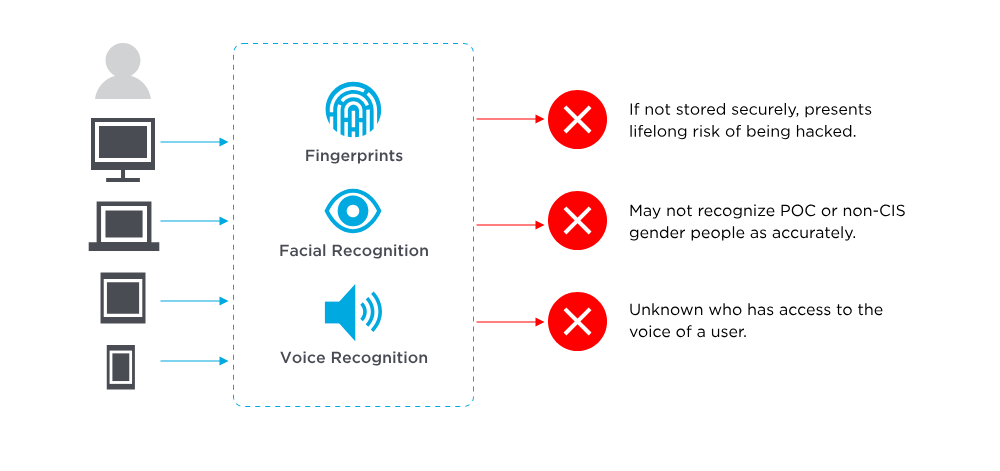
\includegraphics[width=1\linewidth]{bio2.png}
    \caption{Negativne strane biometrijske autentikacije.\cite{bio}}
    \label{fig:enter-label}
\end{figure}

\subsection{Adaptivna autentikacija}
\indent Jedan od sofisticiranijih načina koji se koristi zarad olakšavanje pristupa nalozima, dok još uvek očuvava zadovoljavajuć nivo sigurnosti. Pri prijavljivanju, razni faktori su analizirani (geolokacija, vreme prijavljivanja, korišćeni uređaj...) i poređeni sa uobičajenim ponašanjima asociranim sa korisnikom. Ovom analizom se kvantifikuje ``rizik'' neovlašćenog pristupanja nalogu, i shodno sa nivoom rizika traži se više slojeva autentikacije. Primera radi, ako se korisnik prijavljuje iz njihovog doma, sa prethodno korišćenih uređaja tokom vremena kada uglavnom koriste dati nalog, kvantifikovani rizik će imati nisku vrednost i dopustiti prijavu korišćenjem samo korisničkog imena i šifre. Ako se isti taj korisnik prijavljuje korišćenjem novog uređaja sa nove lokacije, biće zadražeti dodatni koraci poput OTP. U slučajevima da je procenjeni rizik prevelik, moguće je potpuno blokiranje prijvaljivanja. \cite{adaptive}

\begin{figure}[H]
    \centering
    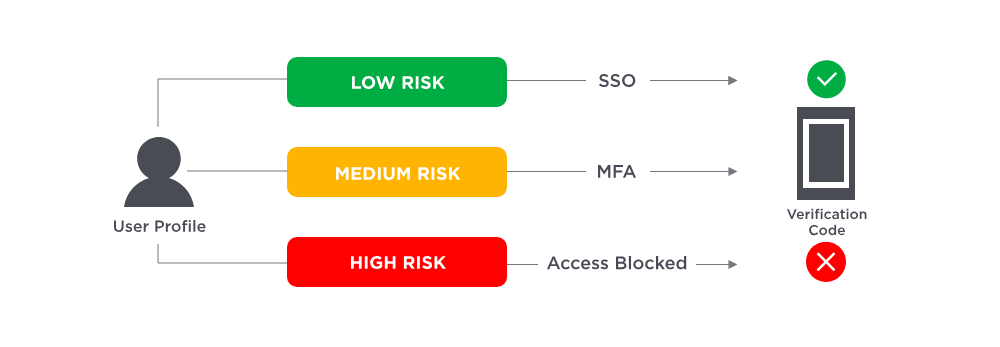
\includegraphics[width=0.8\linewidth]{Adaptive.png}
    \caption{Shema rada sistema adaptive autentikacije.\cite{adaptive}}
    \label{fig:enter-label}
\end{figure}

\newpage
\section{Zaključak}
\indent Bez obzira na veliki značaj sigurnosti lozinki, i samim tim naloga, značajan broj ljudi ovu temu olako shvata i drži se ustaljenih loših praksi poput slabih lozinki, manjka MFA, ponovnog korišćenja istih lozinki i nesigurnog njihovog nesigurnog čuvanja. Nivo tehnološkog obrazovanja nije jak indikator boljih sigurnosnih praksi korisnika. Najveći napredak u sigurnosti koji korisnici mogu da naprave je korišćenje menadžera lozinki (npr. KeePassXC) i MFA metoda (poput OTP i biometrijske autentikacije). Fokus eksperata sajber sigurnosti treba biti okrenut ka kreiranju sistema koji su sigurni sa što manje trenja sa korisničke strane, jer je to trenje glavni razlog manje sigurnosti. 
\bibliography{bib}
\end{document}